\documentclass[12pt, oneside,a4paper]{article}   	% use "amsart" instead of "article" for AMSLaTeX format

\usepackage{graphicx}
\graphicspath{ {\string} }
\usepackage{subcaption}

\usepackage{tabularx}   

%%%%%%%%%%%%%%%%%%%%%%%%%%%%%%%%%%%%%%%%%%%%%%%%%%%%
% set up packages
%%%%%%%%%%%%%%%%%%%%%%%%%%%%%%%%%%%%%%%%%%%%%%%%%%%%
\usepackage{geometry}                
\usepackage{textcomp}                
\usepackage{amsmath}                
\usepackage{graphicx}                
\usepackage{amssymb}                
\usepackage{fancyhdr}                
\usepackage{subcaption}                
\usepackage{bm}                
\usepackage{lineno}
% package for comments
\usepackage{soul}
\sethlcolor{lightgray}

\usepackage{wrapfig}

\usepackage[usenames, dvipsnames]{color}

\usepackage[breaklinks=true]{hyperref}
\hypersetup{
    colorlinks=true,
    linkcolor=red,
    filecolor=orange,      
    urlcolor=red,
    citecolor=Violet,
}

\usepackage[superscript,noadjust]{cite} % puts dash in citations to abbreviate
\usepackage [autostyle, english = american]{csquotes} % sets US-style quotes

\usepackage{etoolbox} % block quotes

\usepackage{float}

\usepackage{pgf}
\usepackage{tikz}
\usepackage{eqnarray}

\usepackage{listings} % code blocks
\usepackage{setspace}

\usepackage{lscape}

\usepackage{natbib}
%\bibliographystyle{abbrvnat}
\setcitestyle{authoryear}

% Adds parentheses around year
%\setcitestyle{authoryear,open={(},close={)}}

%%%%%%%%%%%%%%%%%%%%%%%%%%%%%%%%%%%%%%%%%%%%%%%%%%%%
% call packages
%%%%%%%%%%%%%%%%%%%%%%%%%%%%%%%%%%%%%%%%%%%%%%%%%%%%	
\geometry{letterpaper, marginparwidth=60pt} % sets up geometry              		
\linenumbers % adds line numbers 
\MakeOuterQuote{"} % sets quote style
\doublespacing % setspace

%%%%%%%%%%%%%%%%%%%%%%%%%%%%%%%%%%%%%%%%%%%%%%%%%%%%
% patches with etoolbox 
%%%%%%%%%%%%%%%%%%%%%%%%%%%%%%%%%%%%%%%%%%%%%%%%%%%%	
% block quotes
\AtBeginEnvironment{quote}{\small}

% linenumbers
\makeatletter
\patchcmd{\@startsection}{\@ifstar}{\nolinenumbers\@ifstar}{}{}
\patchcmd{\@xsect}{\ignorespaces}{\linenumbers\ignorespaces}{}{}
\makeatother

%%%%%%%%%%%%%%%%%%%%%%%%%%%%%%%%%%%%%%%%%%%%%%%%%%%%
% tikzlibrary modifications
%%%%%%%%%%%%%%%%%%%%%%%%%%%%%%%%%%%%%%%%%%%%%%%%%%%%	
\usetikzlibrary{fit}
\usetikzlibrary{positioning}
\usetikzlibrary{arrows}
\usetikzlibrary{automata}

%%%%%%%%%%%%%%%%%%%%%%%%%%%%%%%%%%%%%%%%%%%%%%%%%%%%
% page formatting; exact 1 in margins
%%%%%%%%%%%%%%%%%%%%%%%%%%%%%%%%%%%%%%%%%%%%%%%%%%%%
\pagestyle{plain}                                                     

\setlength{\textwidth}{6.5in}    
\setlength{\oddsidemargin}{0in}
\setlength{\evensidemargin}{0in}
\setlength{\textheight}{8.5in}
\setlength{\topmargin}{0in}
\setlength{\headheight}{0in}
\setlength{\headsep}{0in}
\setlength{\footskip}{.5in}

%%%%%%%%%%%%%%%%%%%%%%%%%%%%%%%%%%%%%%%%%%%%%%%%%%%%
% defining code blocks using listings package
%%%%%%%%%%%%%%%%%%%%%%%%%%%%%%%%%%%%%%%%%%%%%%%%%%%%

\definecolor{dkgreen}{rgb}{0,0.6,0}
\definecolor{gray}{rgb}{0.5,0.5,0.5}
\definecolor{mauve}{rgb}{0.58,0,0.82}

\lstset{frame=tb,
  language=R,
  aboveskip=3mm,
  belowskip=3mm,
  showstringspaces=false,
  columns=flexible,
  basicstyle={\small\ttfamily},
  numbers=none,
  numberstyle=\tiny\color{gray},
 % keywordstyle=\color{blue},
  commentstyle=\color{dkgreen},
  stringstyle=\color{mauve},
  breaklines=true,
  breakatwhitespace=true,
  tabsize=3,
  otherkeywords={0,1,2,3,4,5,6,7,8,9},
  deletekeywords={data,frame,length,as,character,dunif,ps},
}

%%%%%%%%%%%%%%%%%%%%%%%%%%%%%%%%%%%%%%%%%%%%%%%%%%%%
%%%%%%%%%%%%%%%%%%%%%%%%%%%%%%%%%%%%%%%%%%%%%%%%%%%%
% begin document
%%%%%%%%%%%%%%%%%%%%%%%%%%%%%%%%%%%%%%%%%%%%%%%%%%%%
%%%%%%%%%%%%%%%%%%%%%%%%%%%%%%%%%%%%%%%%%%%%%%%%%%%%

\begin{document}

% Initial conditions: P=1, V=1 
\begin{figure}[h]
	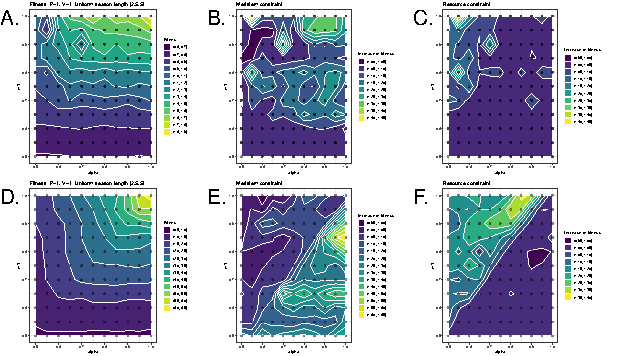
\includegraphics[page=1,width=\textwidth]{figure-1} % 
        \caption{ Initial conditions are $P=1, V=1, I=0, F=0$. The panels are (A-C) no branching ($\gamma=0$), and (D-F) all of the meristem divisions generate branches ($\gamma=1$). Without branching, fitness primarily increases via increases to the meristem division rate ($m$). With branching, fitness increases both as meristem division rate and resource use efficiency increase. \hl{I've reduced the range of parameter values so that end of season fitness is now 6 rather than 40 when I included values up to $m=\alpha=1.5$} }
        \label{fig:intro-figure}
\end{figure}

% Initial conditions: variable 0
\begin{figure}[h]
	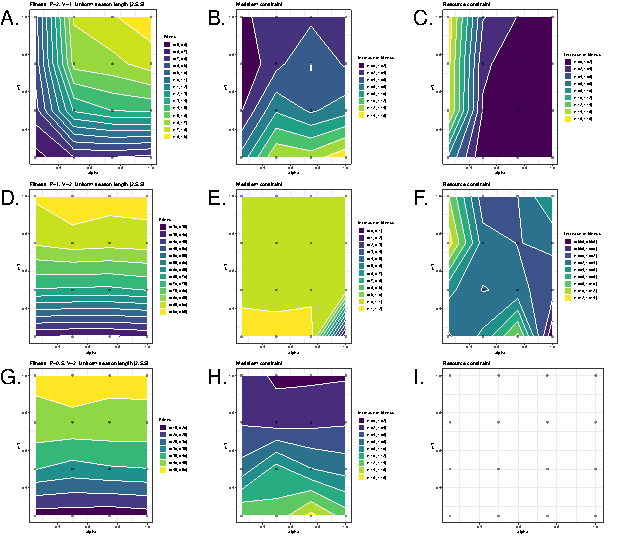
\includegraphics[page=1,width=\textwidth]{figure-2} % 
        \caption{ In all panels, there is no branching ($\gamma=0$) but the initial conditions vary. The panels are (A-C) have a 2:1 primary meristem to vegetative biomass ratio, (D-F) have a 1:2 primary meristem to vegetative biomass ratio, and (G-I) have a 1:4 primary meristem to vegetative biomass ratio (\hl{Error in plotting the effect of relaxing resource constraint.}). As the initial ratio of vegetative biomass increases, the effect of increasing resource use efficiency or relaxing the resource constraint  becomes weaker. This effect is visible both by the flattening of the fitness curves (compare A to D \& G) and the weak sensitivity of fitness to relaxing resource constraints (panels F \& I). With a 2:1 primary meristem to vegetative biomass ratio, the effect of relaxing constraints is shifted away from the 1:1 line such that the strongest sensitivity is for values smaller values of $m$ or $\alpha$, when compared to Figure 1. }
        \label{fig:intro-figure}
\end{figure}

% Initial conditions: branching with variable initial conditions
\begin{figure}[h]
	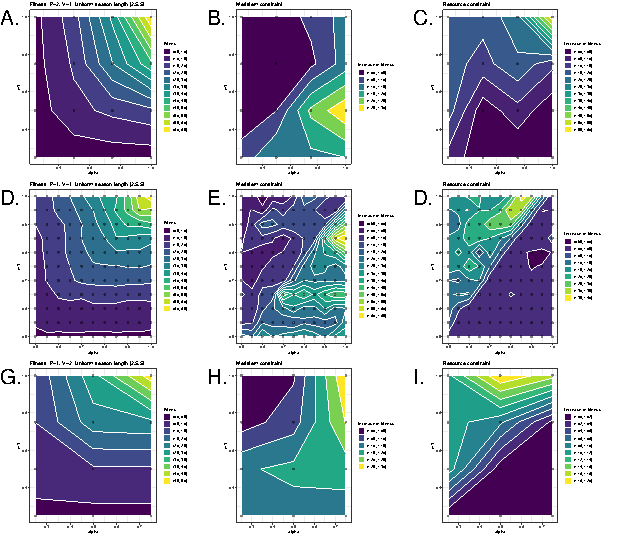
\includegraphics[page=1,width=\textwidth]{figure-3} % 
        \caption{ In all panels, there is branching ($\gamma=1$) but the initial conditions vary. The panels are (A-C) have a 2:1 primary meristem to vegetative biomass ratio, (D-F) have a 1:1 primary meristem to vegetative biomass ratio, and (G-I) have a 1:2 primary meristem to vegetative biomass ratio. As the ratio of vegetative biomass to primary meristems increases (top to bottom), the meristem constraint has the strongest effect closer to the 1:1 line (moving up y axis). Similarly, the resource constraint shifts along the x-axis.   }
        \label{fig:intro-figure}
\end{figure}


\end{document}